\documentclass[border=10pt]{standalone}
\usepackage{tikz}
\usetikzlibrary{positioning, arrows.meta, calc}

\definecolor{coloredge}{HTML}{222222}

\begin{document}
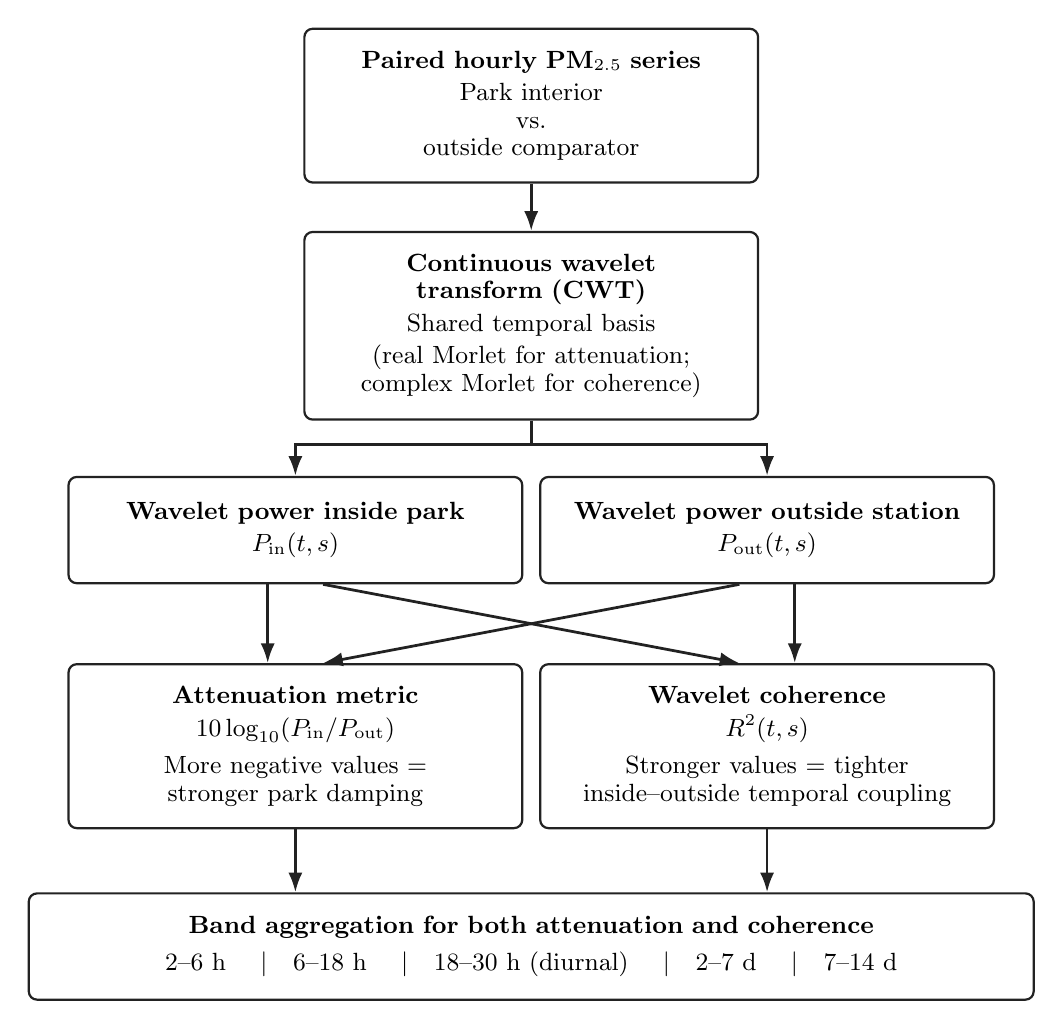
\begin{tikzpicture}[
    % Tighter vertical and horizontal spacing
    node distance=0.8cm and 1.0cm,
    % Clean, unshaded style matching Figure 2
    box/.style={
        rectangle,
        draw=coloredge,
        fill=white,
        rounded corners=3pt,
        align=center,
        text width=5.2cm,
        minimum height=1.35cm,
        inner sep=8pt,
        line width=0.8pt,
        text=black,
        font=\linespread{0.9}\small
    },
    widebox/.style={
        box,
        text width=12.2cm % Slightly widened to fit the "(diurnal)" text smoothly
    },
    arrow/.style={
        -{Latex[length=2.5mm, width=1.8mm]},
        coloredge,
        line width=1.0pt
    }
]

% ==============================
% Row 1 & 2: Input and CWT
% ==============================
\node[box] (input) {
    \textbf{Paired hourly PM$_{2.5}$ series} \\[0.2em]
    Park interior \\
    vs. \\
    outside comparator
};

\node[box, below=0.6cm of input] (cwt) {
    \textbf{Continuous wavelet transform (CWT)} \\[0.2em]
    Shared temporal basis \\[0.2em]
    (real Morlet for attenuation; \\ complex Morlet for coherence)
};

% ==============================
% Row 3: Wavelet Power
% ==============================
% Positioned symmetrically below CWT
\node[box, below left=0.7cm and 0.1cm of cwt.south] (powin) {
    \textbf{Wavelet power inside park} \\[0.2em]
    $P_{\mathrm{in}}(t, s)$
};

\node[box, below right=0.7cm and 0.1cm of cwt.south] (powout) {
    \textbf{Wavelet power outside station} \\[0.2em]
    $P_{\mathrm{out}}(t, s)$
};

% ==============================
% Row 4: Derived Metrics
% ==============================
\node[box, below=1.0cm of powin] (att) {
    \textbf{Attenuation metric} \\[0.2em]
    $10\log_{10}(P_{\mathrm{in}}/P_{\mathrm{out}})$ \\[0.4em]
    More negative values = \\
    stronger park damping
};

\node[box, below=1.0cm of powout] (coh) {
    \textbf{Wavelet coherence} \\[0.2em]
    $R^2(t, s)$ \\[0.4em]
    Stronger values = tighter \\
    inside--outside temporal coupling
};

% ==============================
% Row 5: Band Aggregation
% ==============================
\node[widebox, below=0.8cm of $(att.south)!0.5!(coh.south)$] (bands) {
    \textbf{Band aggregation for both attenuation and coherence} \\[0.4em]
    2--6 h \quad\textbar\quad 6--18 h \quad\textbar\quad 18--30 h (diurnal) \quad\textbar\quad 2--7 d \quad\textbar\quad 7--14 d
};

% ==============================
% Arrows
% ==============================
\draw[arrow] (input) -- (cwt);

% Arrows from CWT branching to Power boxes
\draw[arrow] (cwt.south) -- ++(0,-0.3) -| (powin.north);
\draw[arrow] (cwt.south) -- ++(0,-0.3) -| (powout.north);

% Crossing arrows from Power to Metrics (offset slightly so they don't merge)
\draw[arrow] ([xshift=-10pt]powin.south) -- ([xshift=-10pt]att.north);
\draw[arrow] ([xshift=10pt]powin.south) -- ([xshift=-10pt]coh.north);

\draw[arrow] ([xshift=-10pt]powout.south) -- ([xshift=10pt]att.north);
\draw[arrow] ([xshift=10pt]powout.south) -- ([xshift=10pt]coh.north);

% Arrows from Metrics down to Bands
\draw[arrow] (att.south) -- (att.south |- bands.north);
\draw[arrow] (coh.south) -- (coh.south |- bands.north);

\end{tikzpicture}
\end{document}